In this section we are going to provide a formal description of the system-to-be using the Alloy 6 language. 
We have separated the description in two parts: the first one is the static part, which describes the structure of the system, and the second 
one is the dynamic part, which describes the behavior of the system and how it evolves in time.

\section{Static part}
This model aims to describe the structure of the system, focusing on the main entities and their relationships. In particular, we are going to 
describe the relationships between internships, applications, interviews and users of the platform.

\subsubsection{Signatures}
The following signatures describe the main entities of the system:
\begin{lstlisting}
abstract sig User {}                 // Abstract signature for all users
// Student class to model its submitted applications and participations in internships
sig Student extends User {           
    submits: set Application,        // Applications submitted by student
    participates: set Internship     // Internships student has participated in
}
// Company signature to model companies' published internships
sig Company extends User {
    publishes: set Internship        // Internships published by company
}
// University signature to model universities' students
sig University extends User {
    enrolls: set Student             // Students enrolled in university
}
// Internship signature to model internships' applications and feedbacks
sig Internship {
    submissions: set Application,    // Applications submitted by students for internship
    submittedFeedbacks: set Feedback // Feedbacks submitted by student who participated in internship
}               
// Application signature to model applications' interviews
sig Application {
    interview: lone Interview        // Interview scheduled for application
}
// Feedback signature to model feedbacks submitted by students who participated in internships and companies who published them
sig Feedback {}
// Interview signature to model interviews scheduled for applications
sig Interview {}
\end{lstlisting}

\subsubsection{Facts}
The following facts describe the constraints between the entities and relationships of the system:
\begin{lstlisting}
// Fact to ensure that each application is submitted by only one student (no application can be submitted by multiple students)
fact oneStudentPerApplication{
    all s1,s2: Student | no a: Application | (a in s1.submits and  a in s2.submits and s1 != s2)
}
// Fact to ensure that all applications have been submitted by a student (no orphan applications)
fact allApplicationsInStudent{
    all a: Application | some s: Student | a in s.submits
}
// Fact to ensure that a student cannot submit multiple applications for the same internship
fact noRepeatedApplicationsForSameInternship{
    all s: Student | no i: Internship | 
        (some a1,a2: s.submits | (a1 in i.submissions and a2 in i.submissions and a1 != a2))
}
// Fact to ensure that all internships that a student has participated in have an application submitted by the student
fact allStudentInternshipsHaveApplication{
    all s: Student, i: s.participates | some a: s.submits | a in i.submissions
}
// Fact to ensure that each internship is published by only one company (no internship can be published by multiple companies)
fact oneCompanyPerInternship{
    all c1,c2: Company | no i: Internship | (i in c1.publishes and  i in c2.publishes and c1 != c2)
}
// Fact to ensure that all internships have been published by a company (no orphan internships)
fact allInternshipsInCompany{
    all i: Internship | some c: Company | i in c.publishes
}
// Fact to ensure that each student is enrolled in only one university (no student can be enrolled in multiple universities)
fact oneUniPerStudent{
    all u1,u2: University | no s: Student | (s in u1.enrolls and  s in u2.enrolls and u1 != u2)
}
// Fact to ensure that all students are enrolled in a university (no orphan students)
fact allStudentsInUni{
    all s: Student | some u: University | s in u.enrolls
}
// Fact to ensure that each application is submitted for only one internship (no application can be submitted for multiple internships)
fact oneInternshipPerApplication{
    all i1,i2: Internship | no a: Application | (a in i1.submissions and  a in i2.submissions and i1 != i2)
}
// Fact to ensure that all applications have been submitted for an internship (no orphan applications)
fact allSelectedStudentsApplicationsInInternship{
    all a: Application | some i: Internship | a in i.submissions
}
// Fact to ensure that each feedback is submitted for only one internship (no feedback can be submitted for multiple internships)
fact oneInternshipPerFeedback{
    all i1,i2: Internship | no f: Feedback | (f in i1.submittedFeedbacks and  f in i2.submittedFeedbacks and i1 != i2)
}
// Fact to ensure that all feedbacks have been submitted for an internship (no orphan feedbacks)
fact allFeedbacksInInternship{
    all f: Feedback | some i: Internship | f in i.submittedFeedbacks
}
// Fact to ensure that each interview is scheduled for only one application (no interview can be scheduled for multiple applications)
fact oneApplicationPerInterview{
    all a1,a2: Application | no intv: Interview | (intv in a1.interview and intv in a2.interview and a1 != a2)
}
// Fact to ensure that all interviews have been scheduled for an application (no orphan interviews)
fact allInterviewsInApplication{
    all intv: Interview | some a: Application | intv in a.interview
}
// Fact to ensure that a feedback is submitted only if at least a student has participated in the internship
fact feedbackOnlyIfStudentInInternship{
    all f: Feedback, i: Internship | f in i.submittedFeedbacks implies (some s: Student | i in s.participates and 
        (some a: Application | a in s.submits and a in i.submissions))
}
// Fact to ensure that all internships where a student has participated have an interview scheduled for the application
fact allStudentInternshipsHaveInterviewInApplication{
    all s: Student, i: Internship | i in s.participates implies 
        (some a: Application | a in s.submits and a in i.submissions and 
        (some intv: Interview | intv in a.interview))
}
\end{lstlisting}

\subsubsection{Scenario1 (Predicate 0)}
The following predicate describes a simple scenario with 1 university, 2 students, 2 internships, and 1 company.
Only 1 student participates in an internship (the other one does not), both students submit different number of applications, 
there are no bounds on the number of interviews and feedbacks.
\begin{lstlisting}
pred example0 {
    #University = 1
    #Student = 2
    #Internship = 2
    #Company = 1

    one s: Student | #s.submits = 1
    one s: Student | #s.submits = 2
    one s: Student | #s.participates = 1
    one s: Student | #s.participates = 0
} 
run example0 for 4
\end{lstlisting}
\begin{figure}[H]
    \centering
    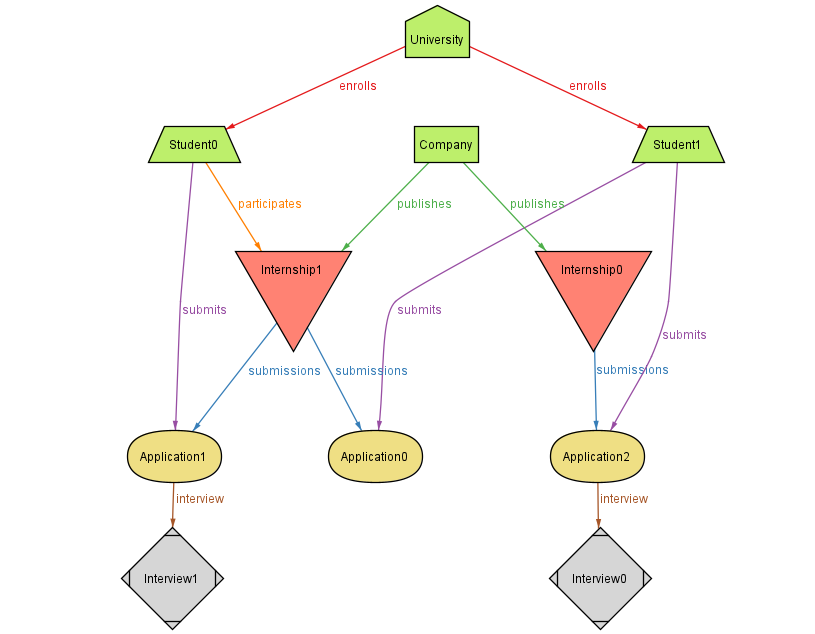
\includegraphics[width=0.75\textwidth]{Images/Alloy/example0.png}
    \caption{World generated by example 0}\label{fig:example0}
\end{figure}

\subsubsection{Scenario2 (Predicate 1)}
The following predicate describes a more structured model with 2 universities, 5 students, 3 internships, and 2 companies.
All students submit more than 1 application, all students participate in less internships than the number of applications they submitted,
at least 1 student participates in an internship, applications and feedbacks are more than 0, and the number of interviews is less than the 
number of applications.
\begin{lstlisting}
pred example1 {
    #University = 2
    #Student = 5
    #Internship = 3
    #Company = 2
    some s: Student | #s.submits > 1
    all s: Student | #s.participates < #s.submits
    some s: Student | #s.participates > 0
    #Application > 0
    #Feedback > 0
    #Interview < #Application
} 
run example1 for 9
\end{lstlisting}
\begin{figure}[H]
    \centering
    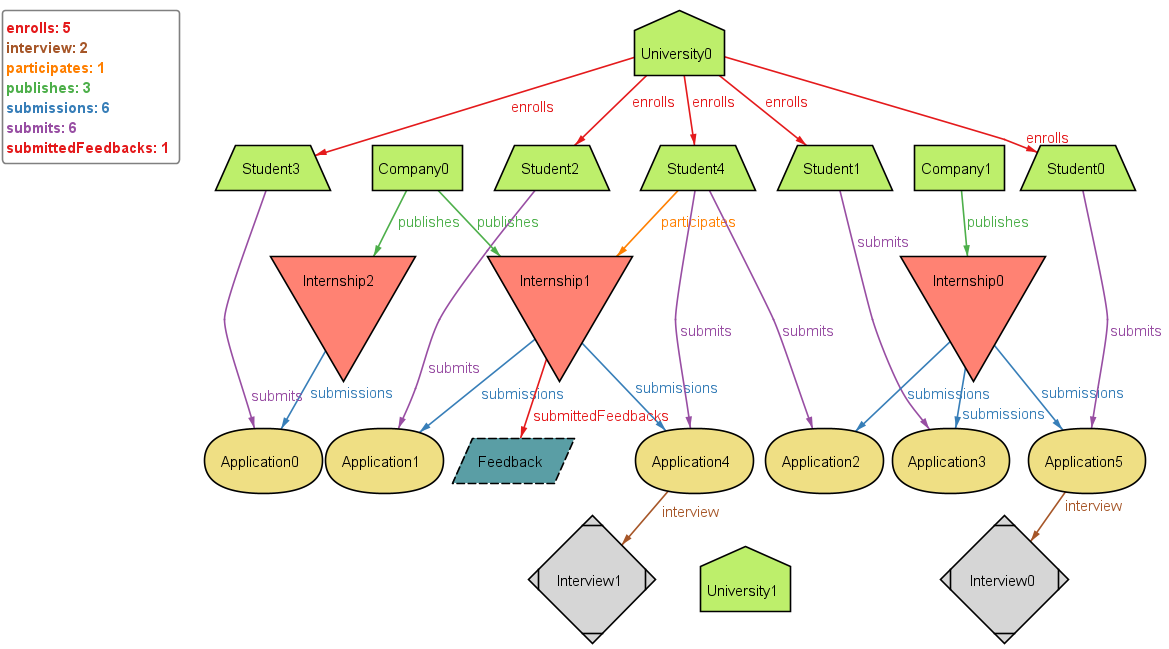
\includegraphics[width=1\textwidth]{Images/Alloy/example1.png}
    \caption{World generated by example 1}\label{fig:example1}
\end{figure}

\subsubsection{Scenario3 (Predicate 2)}
The following predicate describes a more complex model with 2 universities, 5 students, 5 internships, and 2 companies.
All universities have less than 3 students enrolled, at least 1 student submits more than 1 application, 
at least 1 student participates in an internship, at least 1 internship has no submissions,
all internships have less than 3 submitted feedbacks, and the number of submissions is greater than the 
number of students participating. Each company has less than 3 internships published.
\begin{lstlisting}
pred example2 {
    #University = 2     #Student = 5      #Internship = 5   #Company = 2
    #Application > 0    #Feedback > 0     #Interview < #Application
    all u: University | #u.enrolls <= 3
    all u: University | (some s: Student | s in u.enrolls and #s.submits > 0 and #s.participates > 0)
    some s: Student | #s.submits > 1
    all s: Student | #s.submits < 3
    some s: Student | #s.participates > 0
    some s: Student | #s.participates > 1
    some i: Internship | #i.submissions = 0
    all i: Internship | #i.submittedFeedbacks < 3
    all c: Company | #c.publishes <= 3
}
run example2 for 13
\end{lstlisting}
\begin{figure}[H]
    \centering
    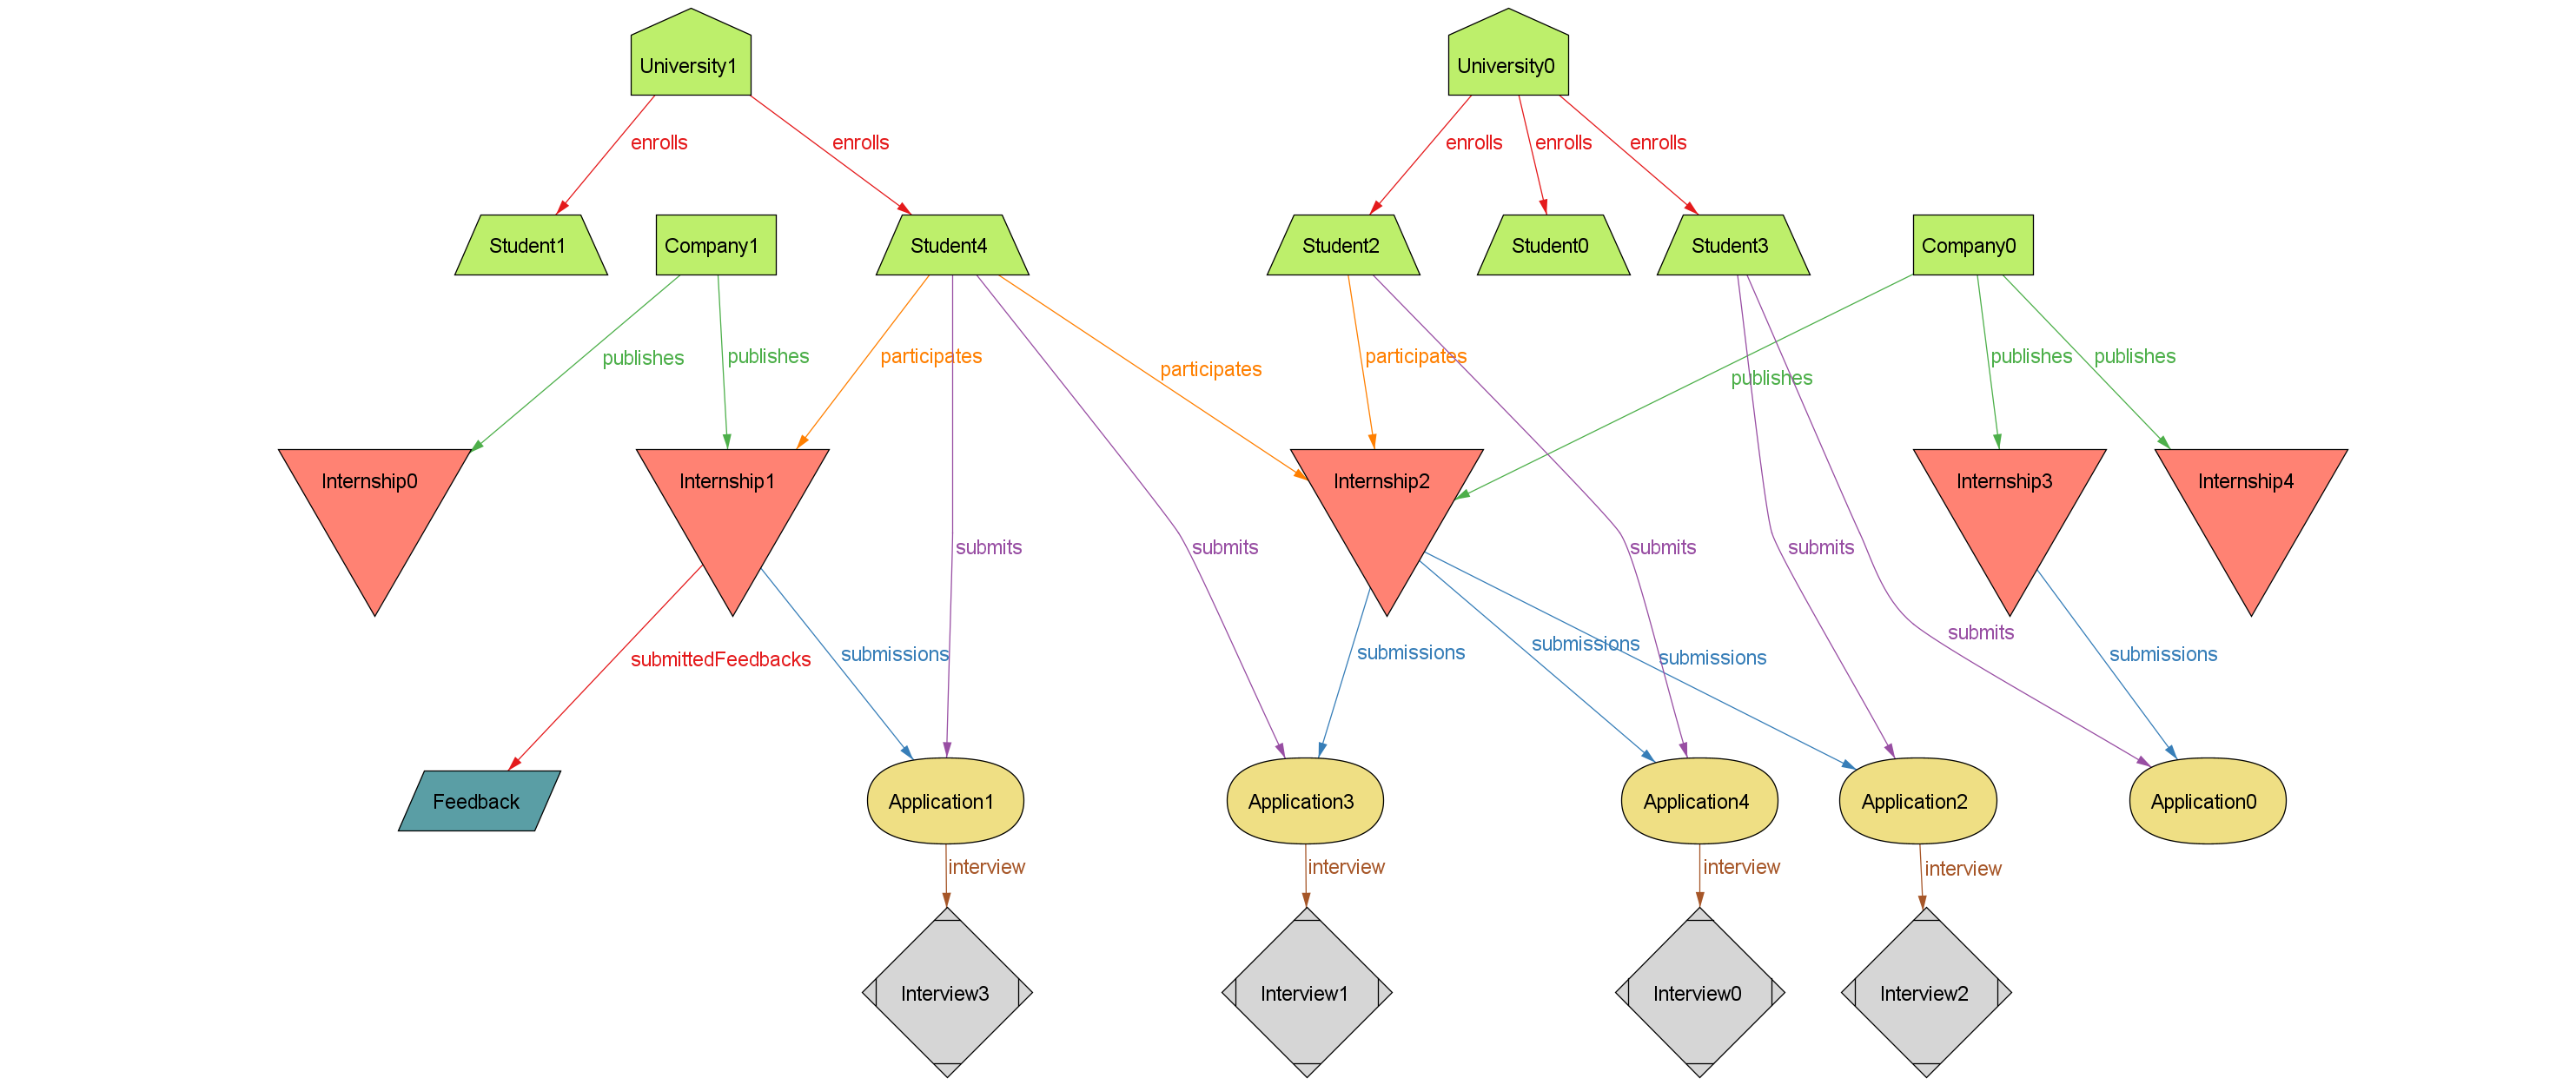
\includegraphics[width=1\textwidth]{Images/Alloy/example2.png}
    \caption{World generated by example 2}\label{fig:example2}
\end{figure}


\section{Dynamic part}
This model aims to describe the behavior of the system, focusing on the evolution of the system in time. In particular, we are going to
describe the evolution of the system when a student submits an application, when a company publishes an internship, when an interview is scheduled,
when a feedback is submitted, and when a student participates in an internship.

\subsubsection{Signatures}
The following signatures describe the main entities of the system:
\begin{lstlisting}
abstract sig User {}
sig Student extends User {
    var submits: set Application,
    var participates: set Internship
}{
    one u: University | this in u.enrolls
}
sig Company extends User {
    var publishes: set Internship
}
sig University extends User {
    var enrolls: set Student
}
var sig Internship {
    var submissions: set Application,
    var submittedFeedbacks: set Feedback,
    var internStatus: one InternshipStatus
}{
    one c: Company | this in c.publishes
}
var sig Application {
   var interview: lone Interview,
   var AppStatus: one ApplicationStatus
}{
    one s: Student | this in s.submits
    one i: Internship | this in i.submissions
}
var sig Feedback {} {
    one i: Internship | this in i.submittedFeedbacks
} 
var sig Interview {} {
    one a: Application | this in a.interview
}
//Model the status of an application
abstract sig ApplicationStatus{}
one sig SubmissionWaiting, SelectedToInterview, AcceptedToInternship, 
AcceptedOffer, RejectedOffer, Rejected extends ApplicationStatus{}
//Model the  status of internship:
abstract sig InternshipStatus{}
one sig InPublishing, InSelection, InProgress, Completed extends InternshipStatus{}
\end{lstlisting}

\subsubsection{Facts}
The following facts describe the constraints between the entities, relationships, and evolution of the system:
\begin{lstlisting}
//Facts used before in Static model 
// Fact to ensure that a student cannot submit multiple applications for the same internship
fact noRepeatedApplicationsForSameInternship{
   always (all s: Student, i: Internship | no disj a1,a2: s.submits | (a1 in i.submissions and a2 in i.submissions) )
}
// Fact to ensure that a feedback is submitted only if at least a student has participated in the internship
fact feedbackOnlyIfStudentInInternship{
    always( all f: Feedback, i: Internship | f in i.submittedFeedbacks 
     implies (some s: Student | i in s.participates and 
        (some a: Application | a in s.submits and a in i.submissions))
    )
}
// Fact to ensure that all internships where a student has participated have an interview scheduled for the application
fact allStudentInternshipsHaveInterviewInApplication{
    always( all s: Student, i: Internship | i in s.participates implies 
        (some a: Application | a in s.submits and a in i.submissions and
        (some intv: Interview | intv in a.interview))
    )
}

//Facts for the dynamic model
// Application can only be in one status at a time
fact ApplicationStatusCanOnlyHaveOnePhaseAtATime{
    always all a: Application | (one a.AppStatus and
    (a.AppStatus = SubmissionWaiting or 
    a.AppStatus = SelectedToInterview or 
    a.AppStatus = AcceptedToInternship or 
    a.AppStatus = AcceptedOffer or 
    a.AppStatus = Rejected or 
    a.AppStatus = RejectedOffer))
}
//Internship can only be in one possible status at a time
fact InternshipStatusCanOnlyHaveOnePhaseAtATime {
    always all i: Internship | one i.internStatus and 
    (i.internStatus = InPublishing or
    i.internStatus = InSelection or
    i.internStatus = InProgress or
    i.internStatus = Completed)
}
// Fact to describe the possible statuses of the applications in each state of the internship
fact allowedAppStatusInEachInternshipStatus {
    always( all i: Internship | 
        (i.internStatus = InPublishing implies 
            (all a: i.submissions | a.AppStatus = SubmissionWaiting)) and 
        (i.internStatus = InSelection implies 
            (all a: i.submissions | a.AppStatus = SelectedToInterview or a.AppStatus = Rejected or a.AppStatus = AcceptedToInternship)) and
        (i.internStatus = InProgress implies 
            (all a: i.submissions | a.AppStatus = AcceptedOffer or a.AppStatus = Rejected or a.AppStatus = RejectedOffer) and (some a: i.submissions | a.AppStatus = AcceptedOffer)) and 
        (i.internStatus = Completed implies  
            (all a: i.submissions | a.AppStatus = AcceptedOffer or a.AppStatus = Rejected or a.AppStatus = RejectedOffer) and (some a: i.submissions | a.AppStatus = AcceptedOffer))
    )
}
// Variation of Interview in every state of the application
fact InterviewInEveryStateOfApplication{
    always all a: Application | 
    (a.AppStatus = SubmissionWaiting implies a.interview = none) and
    (a.AppStatus = SelectedToInterview implies a.interview != none) and
    (a.AppStatus = AcceptedToInternship implies a.interview != none) and
    (a.AppStatus = AcceptedOffer implies a.interview != none) and
    (a.AppStatus = RejectedOffer implies a.interview != none) and
    ((a.AppStatus = Rejected and a.interview != none) implies after always a.interview != none) and
    ((a.AppStatus = Rejected and a.interview = none) implies after always a.interview = none)
}
// When an interview is scheduled for an application, it should never be removed
fact InInterviewCanNotBeRemoved{
    always all a: Application | a.interview != none implies (a.interview' = a.interview)
}
// Student cannot change the university that he is enrolled in
fact studentUniversityInvariant{
    always (all s: Student, u:University | s in u.enrolls implies (after always s in u.enrolls))
}
// Internship cannot change the company that published it
fact internshipCompanyInvariant{
    always (all i: Internship, c:Company | i in c.publishes implies (after always i in c.publishes))
}
// Application cannot change the student that submitted it
fact applicationStudentInvariant{
    always (all a: Application, s:Student | a in s.submits implies (after always a in s.submits))
}
// Student cannot remove the internship that he has participated in
fact studentInternshipInvariant{
    always (all s: Student, i:Internship | i in s.participates implies (after always i in s.participates))
}
// Application cannot change the internship that it is submitted for
fact applicationInternshipInvariant{
    always (all a: Application, i:Internship | a in i.submissions implies (after always a in i.submissions))
}
//Feedback cannot change the internship that it is submitted for
fact feedbackInternshipInvariant{
    always (all f: Feedback, i:Internship | f in i.submittedFeedbacks implies (after always f in i.submittedFeedbacks))
}
// Fact to describe the possible status evolution of the internship
fact internshipStatusAllowedEvolution {
    always( no i: Internship | 
        i.internStatus = InPublishing and (i.internStatus' = InProgress or i.internStatus' = Completed)
        or
        i.internStatus = InSelection and (i.internStatus' = InPublishing or i.internStatus' = Completed)
        or
        i.internStatus = InProgress and (i.internStatus' = InSelection or i.internStatus' = InPublishing)
        or
        i.internStatus = Completed and (i.internStatus' = InSelection or i.internStatus' = InProgress or i.internStatus' = InPublishing)
    )
}
// Fact to describe the possible status evolution of the application
fact allowedAppEvol {
    always (no a: Application | 
        a.AppStatus = SubmissionWaiting and (a.AppStatus' = AcceptedOffer or a.AppStatus' = RejectedOffer or a.AppStatus' = AcceptedToInternship)
        or
        a.AppStatus = SelectedToInterview and (a.AppStatus' = AcceptedOffer or a.AppStatus' = RejectedOffer or a.AppStatus' = SubmissionWaiting)
        or
        a.AppStatus = AcceptedToInternship and (a.AppStatus' = Rejected or a.AppStatus' = SelectedToInterview or a.AppStatus' = SubmissionWaiting)
        or
        a.AppStatus = AcceptedOffer and (a.AppStatus' = Rejected or a.AppStatus' = RejectedOffer or a.AppStatus' = AcceptedToInternship or a.AppStatus' = SelectedToInterview or a.AppStatus' = SubmissionWaiting)
        or
        a.AppStatus = RejectedOffer and (a.AppStatus' = Rejected or a.AppStatus' = AcceptedOffer or a.AppStatus' = AcceptedToInternship or a.AppStatus' = SelectedToInterview or a.AppStatus' = SubmissionWaiting)
        or
        a.AppStatus = Rejected and (a.AppStatus' = AcceptedOffer or a.AppStatus' = RejectedOffer or a.AppStatus' = AcceptedToInternship or a.AppStatus' = SelectedToInterview or a.AppStatus' = SubmissionWaiting)
    )
}
// An internship in publishing or selection cannot have students participating in it and feedbacks submitted
fact NoStudentsOrFeedbacksInInternshipInPublishingOrSelection{
    always all i: Internship | (i.internStatus = InPublishing or i.internStatus = InSelection) implies
    (no s: Student | i in s.participates) and (no f: Feedback | f in i.submittedFeedbacks)
}
// When internship is in publishing status, no applications submitted should have an interview scheduled
fact noInterviewsWhileInternshipInPublishing {
    always all i: Internship | i.internStatus = InPublishing implies (no a: i.submissions | a.interview != none)
}
// An application can be submitted to the internship only if the internship is in publishing status
fact SubmissionsMutableOnlyInPublishing {
    always all i: Internship | (i.internStatus != InPublishing or i.internStatus' != InPublishing) implies (i.submissions' = i.submissions)
}
// An internship can be in selection status only if at least one application has been submitted
fact InternshipInSelectionOnlyIfApplicationSubmitted{
    always all i: Internship | i.internStatus = InSelection implies (some a: Application | a in i.submissions)
}
// All applications of an internship in selection move from state SelectedToInterview to AcceptedToInternship (or Rejected) at the same step
fact NoSimultaneousSelectedAndAccepted {
    always all i: Internship | (i.internStatus = InSelection and some a: i.submissions | a.AppStatus = AcceptedToInternship) implies (all a: i.submissions | a.AppStatus = AcceptedToInternship or a.AppStatus = Rejected)
}
// If a student participates to an internship, then that internship is in progress or completed
fact NoStudentParticipatesInInternshipIfNotInProgressOrCompleted{
    always all s: Student, i: Internship | i in s.participates implies (i.internStatus = InProgress or i.internStatus = Completed)
}
// An internship can be in progress or completed only if at least one student participates in it
fact InternshipInProgressOrCompletedOnlyIfStudentParticipates{
    always all i: Internship | (i.internStatus = InProgress or i.internStatus = Completed) implies (some s: Student | i in s.participates)
}
// When an internship is in progress status or completed status, all applications should be in the final status: accepted offer, rejected offer or rejected
fact InternshipInProgressOrCompletedApplicationsInFinalStatus{
    always all i: Internship | (i.internStatus = InProgress or i.internStatus = Completed) implies
    (all a: i.submissions | (a.AppStatus = AcceptedOffer or a.AppStatus = RejectedOffer or a.AppStatus = Rejected))
}
// Every Student can only do one internship at a time
fact StudentCanDoOneInternshipsAtATime{
    always all s: Student | let concurrentParticipations = #(s.participates & {i: s.participates | i.internStatus = InProgress}) |
    concurrentParticipations <= 1
}
// Student application number should be more or equals to the number of internships they participated in
fact StudentApplicationsMoreThanParticipations{
    always all s: Student | #s.submits >= #s.participates 
}
// Student should have the offer accepted equal or less than the number of applications submitted and equal to the number of participations
fact StudentOffersAccepted{
    always all s: Student | 
    let numOffersAccepted = #(s.submits & {a: s.submits | a.AppStatus = AcceptedOffer}) |
    let numApplications = #s.submits |
    let numParticipations = #s.participates |
    numOffersAccepted <= numApplications and numOffersAccepted = numParticipations
}
// Student has participated if and only if he accepted the application related to the internship
fact StudentParticipatesInInternship{
    always all s: Student, i: Internship | i in s.participates implies
    (some a: Application | a in s.submits and a in i.submissions and a.AppStatus = AcceptedOffer)
}
// When an internship is in progress or completed, no more interviews should be scheduled
fact noChangeInInterviewsWhenInternshipInProgressOrCompleted{
    always all i: Internship | (i.internStatus = InProgress or i.internStatus = Completed) implies
    i.submissions.interview' = i.submissions.interview
}
// Once Internship is completed, no more feedbacks can be submitted
fact InternshipCompletedNoMoreFeedbacks{
    always all i: Internship | i.internStatus' = Completed implies (i.submittedFeedbacks' = i.submittedFeedbacks)
}
// Once Internship is in progress, feedbacks can be submitted
fact InProgressForFeedbacks{
    always all i: Internship | (#i.submittedFeedbacks' > #i.submittedFeedbacks) implies i.internStatus = InProgress
}
// Once Internship is completed, there should be at least 2 feedbacks
fact AtLeast2FeedbackIfCompleted{
    always all i: Internship | i.internStatus' = Completed implies (#i.submittedFeedbacks > 1)
}

//Initialization
// Forcing the initial state of the system
fact init {
    #University = 1
    #Company = 1
    #Student = 4
    #Internship = 1
    all i: Internship | i.internStatus = InPublishing
}
\end{lstlisting}

\subsubsection{Predicates and Scenario}
In this section we are going to describe the evolution of the system in time, 
focusing on the main actions that can be performed by the users of the system.

\begin{lstlisting}
// Predicates to model the creation of an internship
pred internshipCreation {
    eventually (#Internship = 2 and all i: Internship | i.internStatus = InPublishing and after always #Internship = 2) and 
	always (all a: Application, i: Internship | (a in i.submissions and a.AppStatus = SubmissionWaiting) implies before i.internStatus = InPublishing)
}
// Predicates to model the submission of an application
pred applicationSubmission {
    eventually (some a: Application, s: Student, i: Internship | a in s.submits and a in i.submissions and a.AppStatus = SubmissionWaiting) and eventually #Application > 2
}
// Predicates to model the rejection of an application
pred applicationRejection {
    eventually (some s: Student, i: Internship, a: Application  | a in s.submits and a in i.submissions and a.AppStatus = Rejected)
}
// Predicates to model the selection of an application
pred applicationSelection {
    eventually (some s: Student, i: Internship, a: Application  | a in s.submits and a in i.submissions and a.AppStatus = SelectedToInterview)
}
// Predicates to model the acceptance of an application
pred applicationAcceptance {
    eventually (some s: Student, i: Internship, a: Application  | a in s.submits and a in i.submissions and a.AppStatus = AcceptedToInternship)
}
// Predicates to model the acceptance of an internship
pred internshipAcceptance {
    eventually (some s: Student, i: Internship, a: Application  | a in s.submits and a in i.submissions and a.AppStatus = AcceptedOffer)
}
// Predicates to model the rejection of an internship
pred internshipRejection {
    eventually (some s: Student, i: Internship, a: Application  | a in s.submits and a in i.submissions and a.AppStatus = RejectedOffer)
}
// Predicates to model the submission of a feedback
pred feedbackSubmission {
    eventually (some f: Feedback, i: Internship | f in i.submittedFeedbacks)
}
// Predicates to model the completion of all internships
pred allInternshipCompleted {
    eventually (all i: Internship | i.internStatus = Completed)
}
// RUN THE SYSTEM
run { internshipCreation;applicationSubmission;applicationRejection;
    applicationSelection;applicationAcceptance;internshipAcceptance;
    internshipRejection;feedbackSubmission;allInternshipCompleted 
} for 7
\end{lstlisting}

\begin{figure}
    \centering
    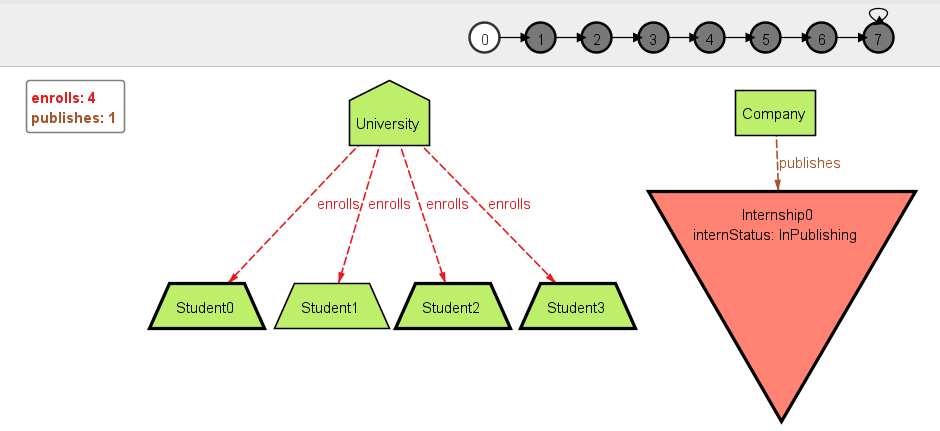
\includegraphics[width=1\textwidth]{Images/Alloy/dyn1.png}\label{fig:dyn1}
\end{figure}
\begin{figure}
    \centering
    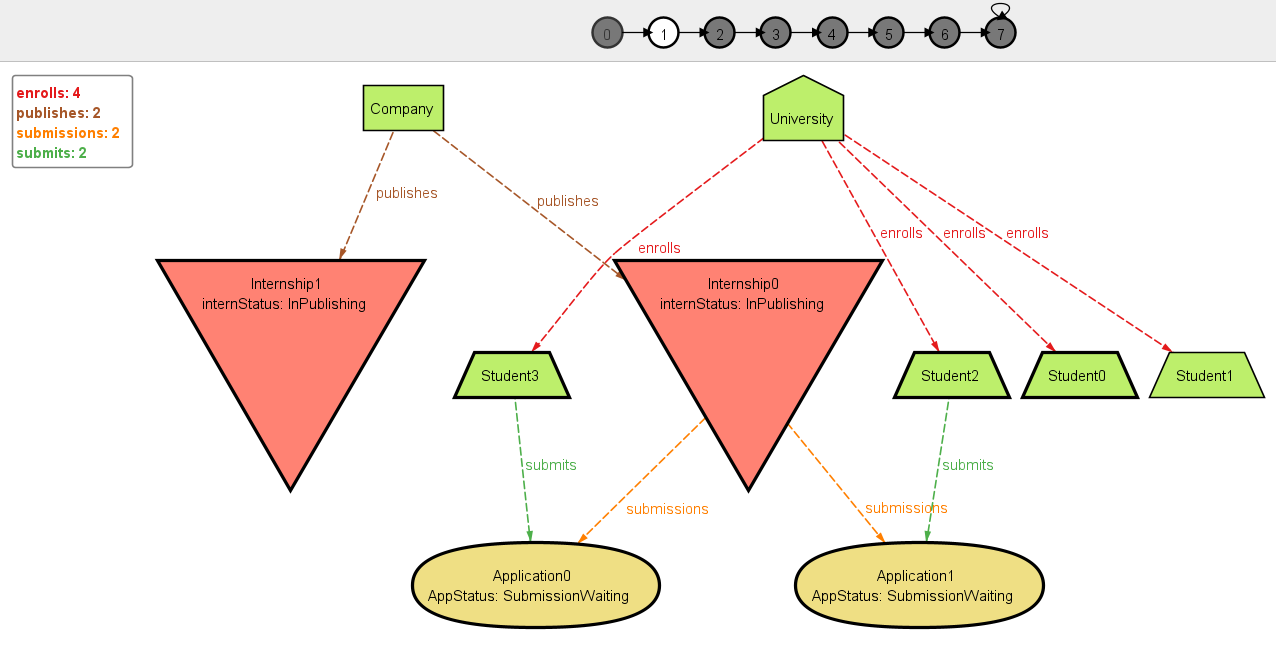
\includegraphics[width=1\textwidth]{Images/Alloy/dyn2.png}\label{fig:dyn2}
\end{figure}
\begin{figure}
    \centering
    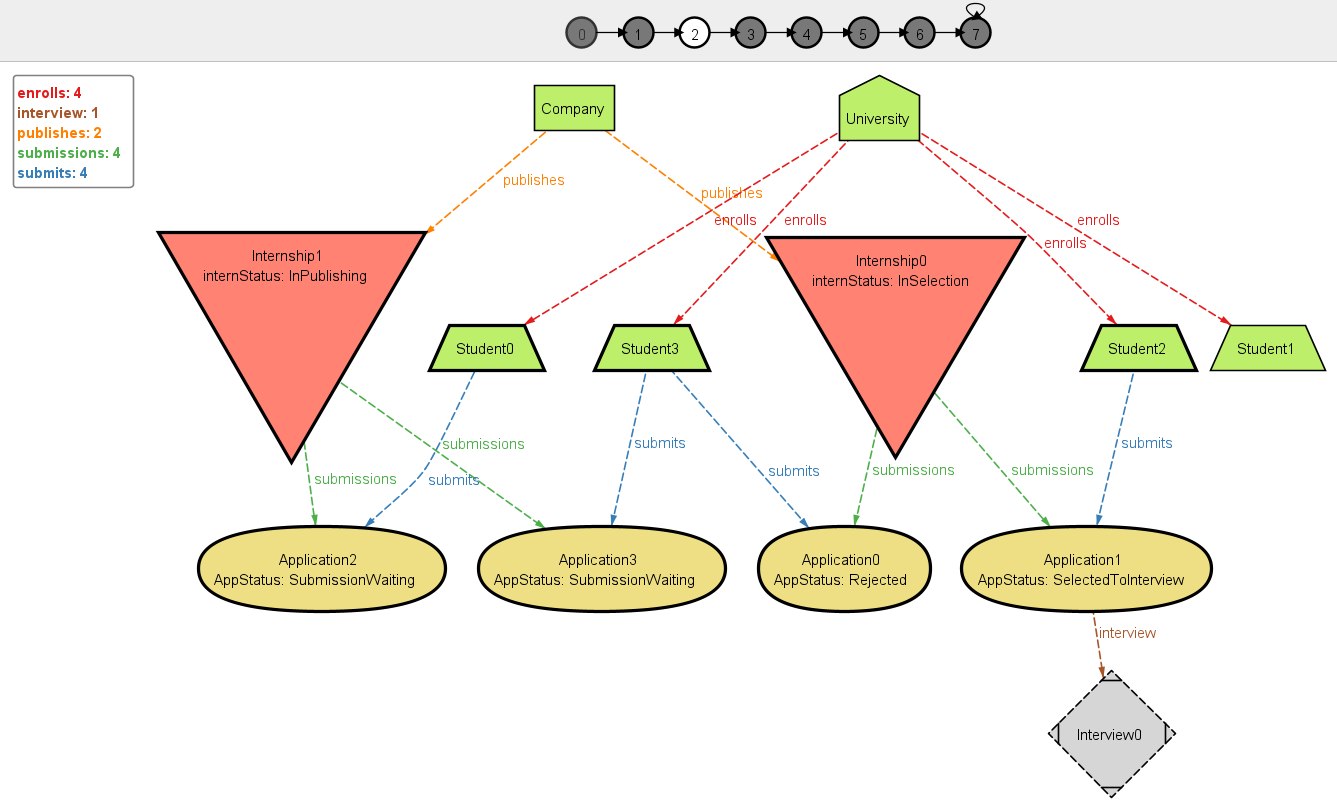
\includegraphics[width=1\textwidth]{Images/Alloy/dyn3.png}\label{fig:dyn3}
\end{figure}
\begin{figure}
    \centering
    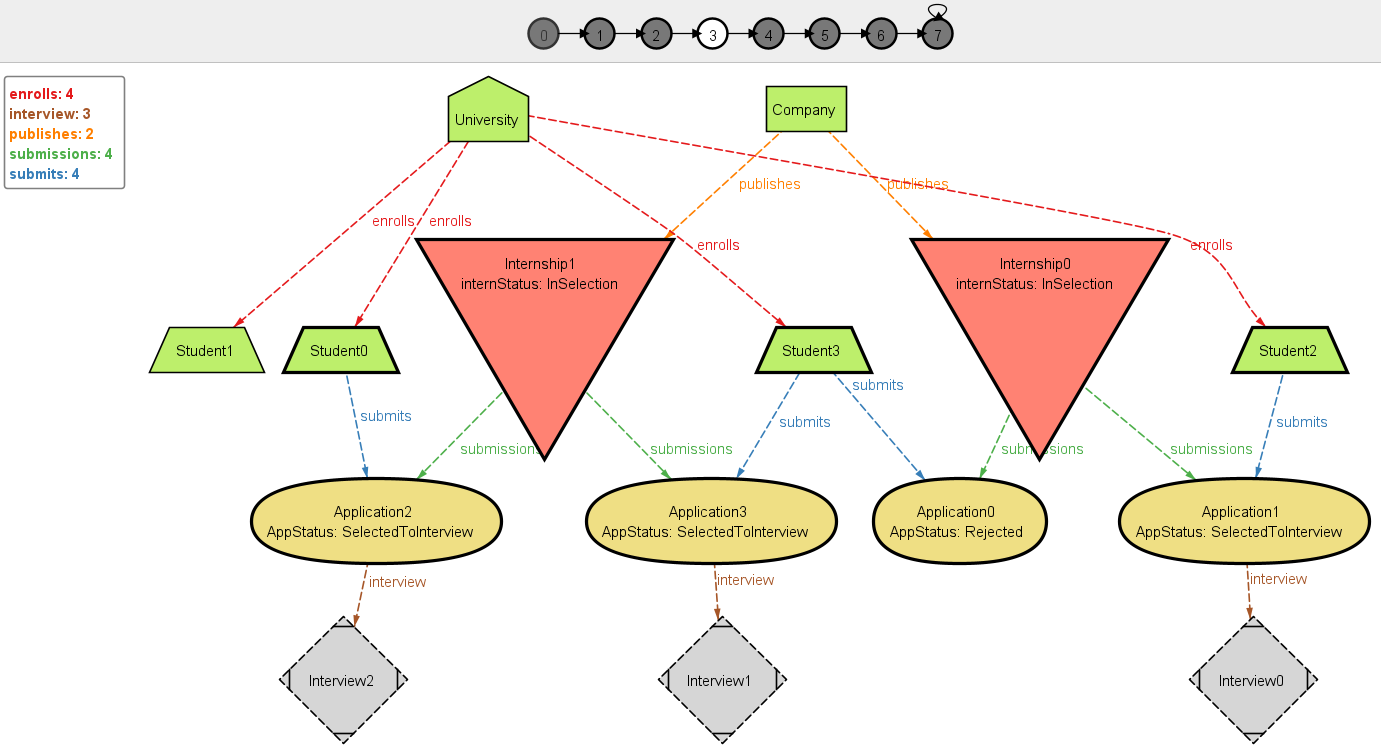
\includegraphics[width=1\textwidth]{Images/Alloy/dyn4.png}\label{fig:dyn4}
\end{figure}
\begin{figure}
    \centering
    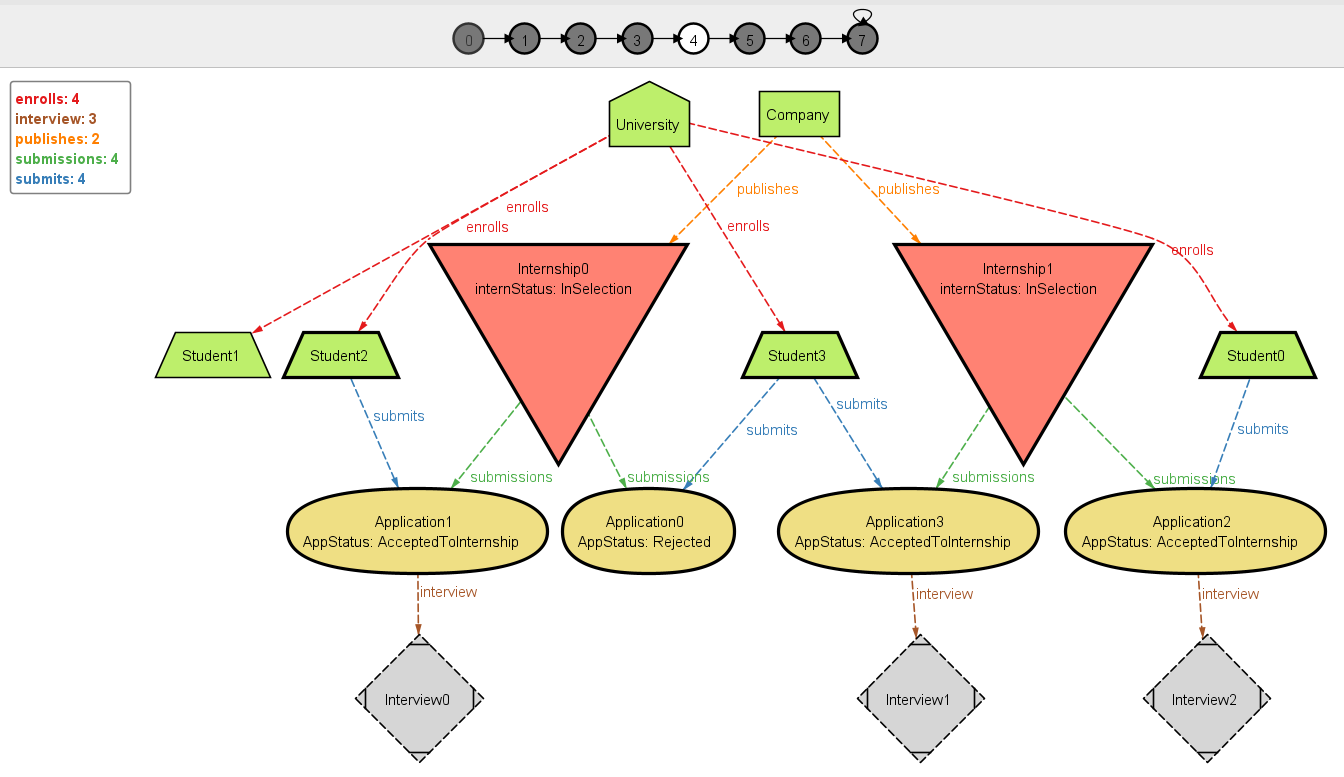
\includegraphics[width=1\textwidth]{Images/Alloy/dyn5.png}\label{fig:dyn5}
\end{figure}
\begin{figure}
    \centering
    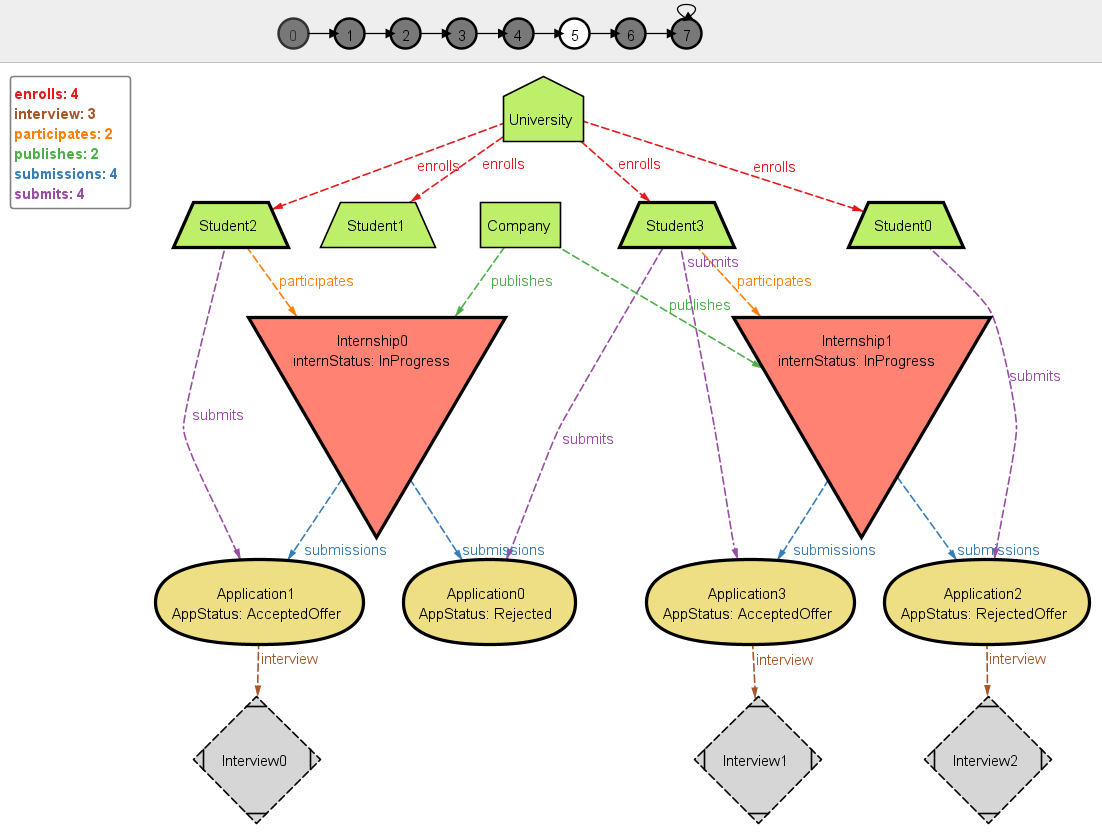
\includegraphics[width=1\textwidth]{Images/Alloy/dyn6.png}\label{fig:dyn6}
\end{figure}
\begin{figure}
    \centering
    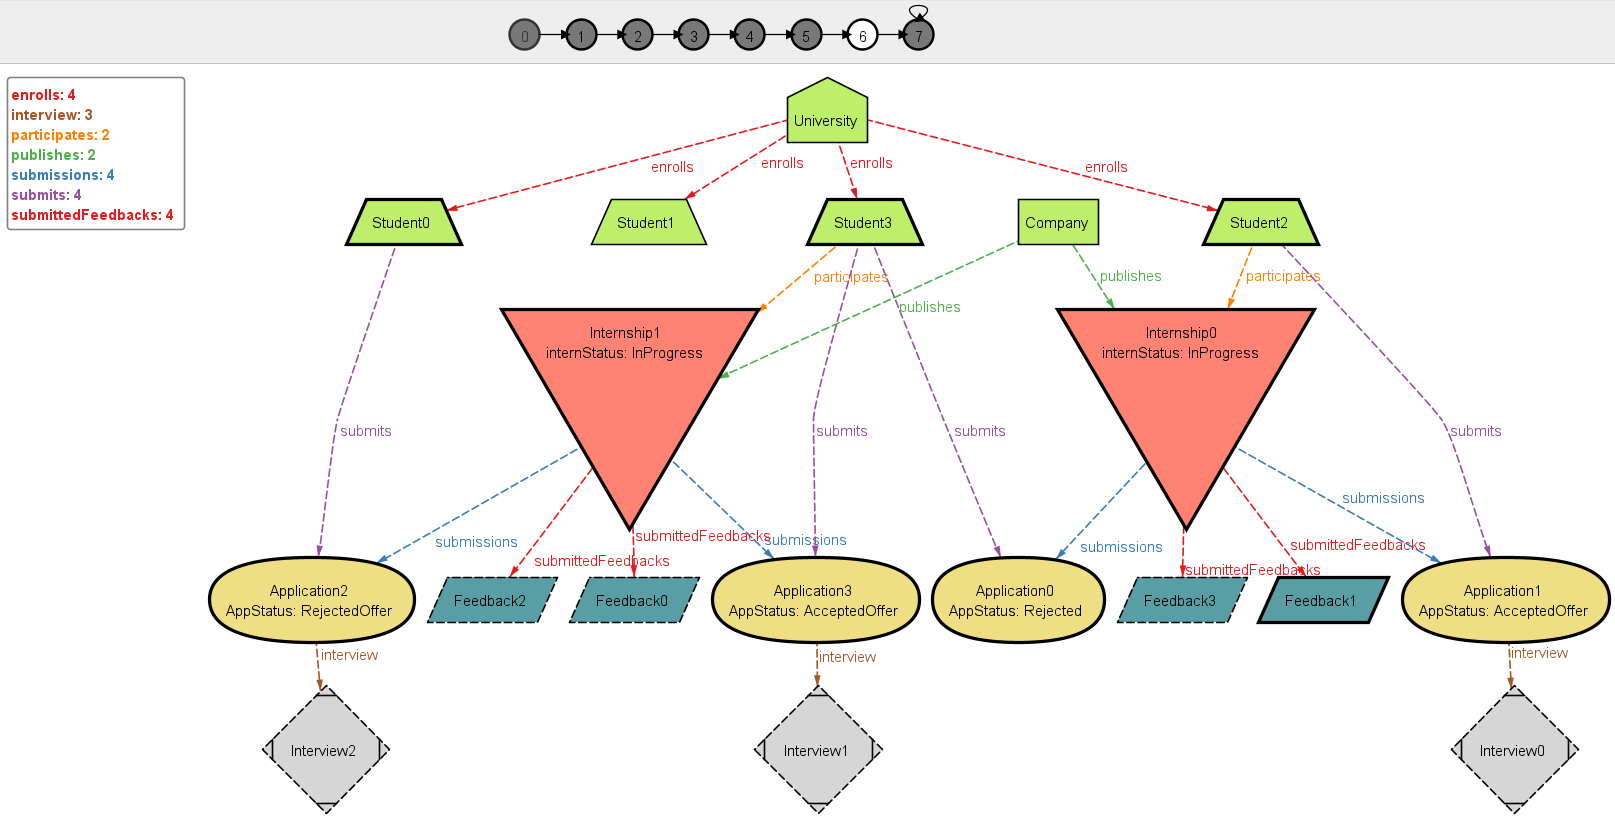
\includegraphics[width=1\textwidth]{Images/Alloy/dyn7.png}\label{fig:dyn7}
\end{figure}
\begin{figure}
    \centering
    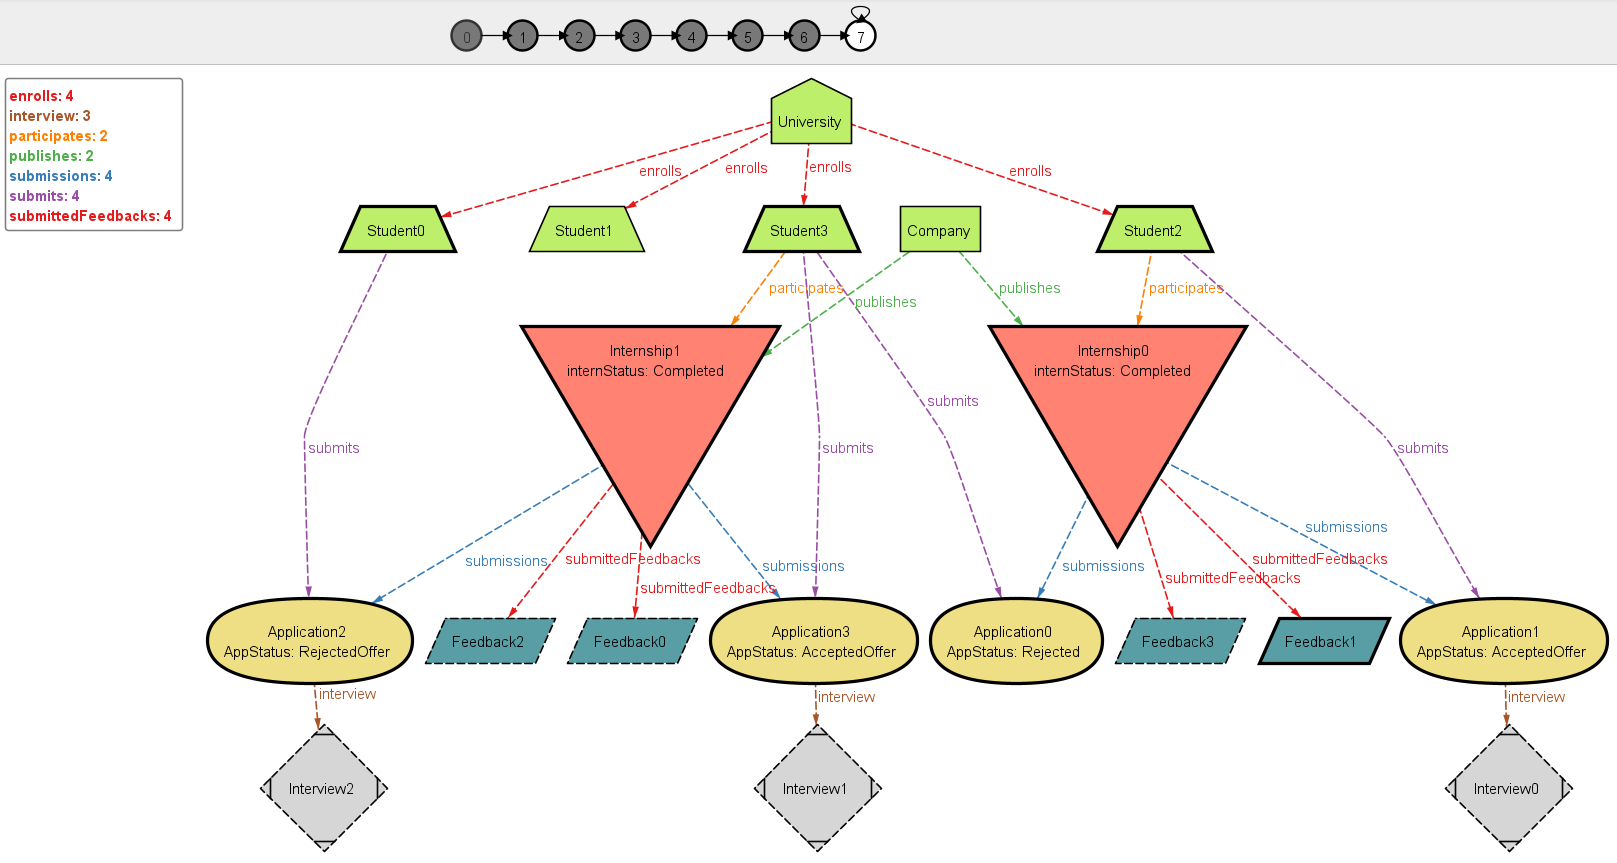
\includegraphics[width=1\textwidth]{Images/Alloy/dyn8.png}\label{fig:dyn8}
\end{figure}